% TikZ 复刻。原图：assets/mercury-spectrum.png
% 回退：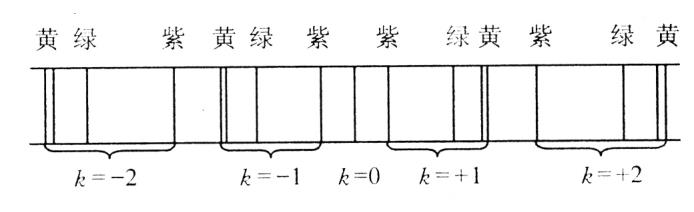
\includegraphics[width=0.92\linewidth]{assets/mercury-spectrum.png}
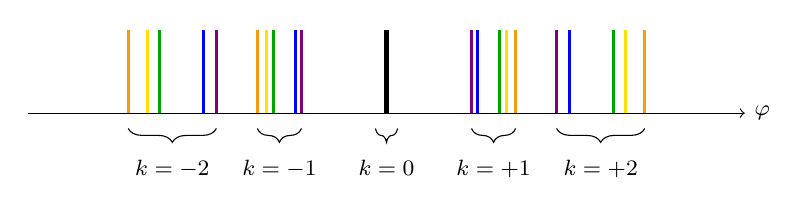
\begin{tikzpicture}[font=\footnotesize, decoration={brace, amplitude=5pt, mirror, raise=1pt}]
  \def\h{1.05}
  \def\yv{1.08}
  \def\yb{1.16}
  \def\yg{1.44}
  \def\yyi{1.52}
  \def\yyii{1.64}
  \draw[->] (-4.55,0) -- (4.55,0);
  \node[right] at (4.55,0) {$\varphi$};
  \draw[line width=2.0pt] (0,0) -- (0,\h);
  \foreach \k in {-2,-1,1,2} {
    \draw[violet, line width=1.05pt] ({\k*\yv},0) -- ({\k*\yv},\h);
    \draw[blue, line width=1.05pt] ({\k*\yb},0) -- ({\k*\yb},\h);
    \draw[green!65!black, line width=1.15pt] ({\k*\yg},0) -- ({\k*\yg},\h);
    \draw[yellow!85!orange, line width=1.1pt] ({\k*\yyi},0) -- ({\k*\yyi},\h);
    \draw[yellow!60!red, line width=1.1pt] ({\k*\yyii},0) -- ({\k*\yyii},\h);
  }
  \draw[decorate] (-2*\yyii,-0.16) -- (-2*\yv,-0.16);
  \node[below=9pt] at (-2*1.36, -0.16) {$k=-2$};
  \draw[decorate] (-\yyii,-0.16) -- (-\yv,-0.16);
  \node[below=9pt] at (-1.36, -0.16) {$k=-1$};
  \draw[decorate] (-0.14,-0.16) -- (0.14,-0.16);
  \node[below=9pt] at (0, -0.16) {$k=0$};
  \draw[decorate] (\yv,-0.16) -- (\yyii,-0.16);
  \node[below=9pt] at (1.36, -0.16) {$k=+1$};
  \draw[decorate] (2*\yv,-0.16) -- (2*\yyii,-0.16);
  \node[below=9pt] at (2*1.36, -0.16) {$k=+2$};
\end{tikzpicture}
